% Author: Izaak Neutelings (March 2020)
\documentclass[border=3pt,tikz]{standalone}
\usepackage{amsmath} % for \dfrac
\usepackage{mathabx} % for \Earth
\usepackage{bm} % \bm
\usepackage{physics}
\usepackage{tikz,pgfplots}
\usepackage[outline]{contour} % glow around text
\usetikzlibrary{angles,quotes} % for pic (angle labels)
\usetikzlibrary{calc}
\usetikzlibrary{decorations.markings}
\tikzset{>=latex} % for LaTeX arrow head
\contourlength{1.6pt}
\usepackage{xcolor}
\colorlet{Ecol}{orange!90!black}
\colorlet{EcolFL}{orange!90!black}
\colorlet{Bcol}{violet!90}
\colorlet{BFcol}{red!60!black}
\colorlet{veccol}{green!45!black}
\colorlet{Icol}{blue!70!black}
\colorlet{pluscol}{red!60!black}
\colorlet{minuscol}{blue!60!black}
\tikzstyle{BField}=[->,thick,Bcol]
\tikzstyle{current}=[->,Icol] %thick,
\tikzstyle{force}=[->,thick,BFcol]
\tikzstyle{vector}=[->,thick,veccol]
\tikzstyle{velocity}=[->,very thick,vcol]
\tikzstyle{charge+}=[very thin,draw=black,top color=red!50,bottom color=red!90!black,shading angle=20,circle,inner sep=0.5]
\tikzstyle{charge-}=[very thin,draw=black,top color=blue!50,bottom color=blue!80,shading angle=20,circle,inner sep=0.5]
\tikzstyle{metal}=[top color=black!15,bottom color=black!25,middle color=black!5,shading angle=10]
\tikzset{
  EFieldLine/.style={thick,EcolFL,decoration={markings,mark=at position #1 with {\arrow{latex}}},
                     postaction={decorate}},
  EFieldLine/.default=0.5,
  BFieldLine/.style={thick,Bcol,decoration={markings,mark=at position #1 with {\arrow{latex}}},
                     postaction={decorate}},
  BFieldLine/.default=0.5,
  pics/Bin/.style={
    code={
      \def\R{0.12}
      \draw[pic actions,#1,line width=0.6] % ,thick
        (0,0) circle (\R) (-135:.7*\R) -- (45:.7*\R) (-45:.7*\R) -- (135:.7*\R);
  }},
  pics/Bout/.style={
    code={
      \def\R{0.12}
      \draw[pic actions,#1,fill=white,line width=0.6] (0,0) circle (\R);
      \fill[pic actions,#1] (0,0) circle (0.3*\R);
  }},
  pics/Bout/.default=Bcol,
  pics/Bin/.default=Bcol,
}



\begin{document}


% B FIELD horizontal, top view
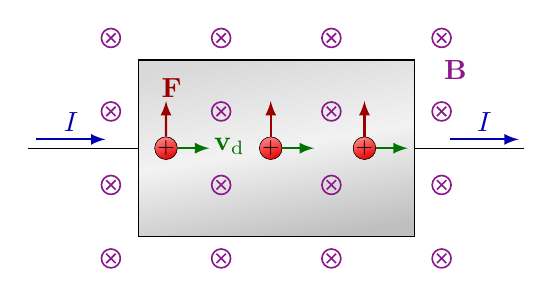
\begin{tikzpicture}
  \def\xmax{3.5}
  \def\ymax{1.4}
  \def\R{0.2}
  \def\Rx{0.26*\ymax}
  \def\H{0.8*\ymax}
  \def\L{\xmax}
  \def\NBy{4}
  \def\NBx{4}
  \coordinate (LT) at (0,\H);
  \coordinate (LB) at (0,-\H);
  \coordinate (RT) at (\L,\H);
  \coordinate (RB) at (\L,-\H);
  \coordinate (Q) at (0.15*\xmax,0.15*\ymax);
  \def\charge#1#2{
    \node[charge+,draw=black,circle,fill,inner sep=0,scale=0.8] (q) at (#1*\xmax,#2*\H) {$+$};
    \draw[vector] (q) --++ (0:0.55);
    \draw[force] (q) --++ (90:0.6);
  }
  
  % CURRENT
  \draw (-0.4*\L,0) -- (0,0);
  \draw (\L,0) -- (1.4*\L,0);
  \draw[metal]
    (LB) rectangle (RT);
  
  % CHARGE
  \charge{0.10}{0.0}
  \charge{0.48}{0.0}
  \charge{0.82}{0.0}
  %\charge{0.14}{0.65}
  %\charge{0.48}{0.65}
  %\charge{0.82}{0.65}
  %\charge{0.14}{-.65}
  %\charge{0.48}{-.65}
  %\charge{0.82}{-.65}
  
  % MAGNETIC FIELD
  \foreach \i [evaluate={\y=(\i-\NBy/2-0.5)*2*\ymax/(\NBy-1);}] in {1,...,\NBy}{
    \foreach \j [evaluate={\x=-0.1*\xmax+(\j-1)*1.2*\xmax/(\NBx-1);}] in {1,...,\NBx}{
      \pic at (\x,\y) {Bin};
    }
  }
  \node[Bcol] at (1.15*\xmax,0.71*\ymax) {$\vb{B}$};
  \node[BFcol] at (0.12*\xmax,0.68*\H) {$\vb{F}$};
  \node[veccol] at (0.33*\xmax,0.02*\H) {$\vb{v}_\mathrm{d}$};
  \draw[->,thick,blue!70!black] ( 1.13*\L,0.1*\H) --++ ( 0.25*\L,0) node[midway,above=-1] {$I$};
  \draw[<-,thick,blue!70!black] (-0.12*\L,0.1*\H) --++ (-0.25*\L,0) node[midway,above=-1] {$I$};
  
\end{tikzpicture}


% B FIELD horizontal, top view
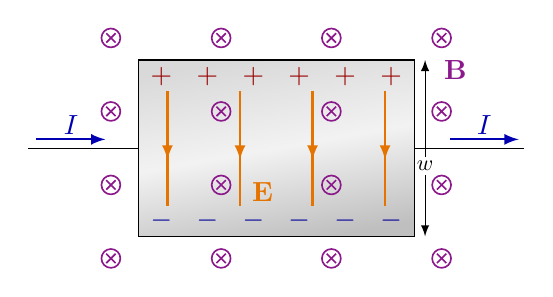
\begin{tikzpicture}
  \def\xmax{3.5}
  \def\ymax{1.4}
  \def\R{0.2}
  \def\Rx{0.26*\ymax}
  \def\H{0.8*\ymax}
  \def\L{\xmax}
  \def\NBy{4}
  \def\NBx{4}
  \def\NE{4}
  \def\NQ{6}
  \coordinate (LT) at (0,\H);
  \coordinate (LB) at (0,-\H);
  \coordinate (RT) at (\L,\H);
  \coordinate (RB) at (\L,-\H);
  \coordinate (Q) at (0.15*\xmax,0.15*\ymax);
  \def\charge#1#2{
    \node[charge+,draw=black,circle,fill,inner sep=0,scale=0.8] (q) at (#1*\xmax,#2*\H) {$+$};
    \draw[vector] (q) --++ (0:0.55);
    \draw[force] (q) --++ (90:0.6);
  }
  
  % CURRENT
  \draw (-0.4*\L,0) -- (0,0);
  \draw (\L,0) -- (1.4*\L,0);
  \draw[<->] (1.04*\L,-\H) --++ (0,2*\H) node[midway,below=3,fill=white,inner sep=2,scale=0.8] {$w$};
  \draw[metal]
    (LB) rectangle (RT);
  
  % ELECTRIC & MAGNETIC FIELD
  \foreach \i [evaluate={\y=(\i-\NBy/2-0.5)*2*\ymax/(\NBy-1);}] in {1,...,\NBy}{
    \foreach \j [evaluate={\x=-0.1*\xmax+(\j-1)*1.2*\xmax/(\NBx-1);}] in {1,...,\NBx}{
      \pic at (\x,\y) {Bin};
    }
  }
  \foreach \i [evaluate={\x=(\i-0.5)*\xmax/\NQ;}] in {1,...,\NQ}{
    \node[pluscol,below=-1]  at (\x, \H) {$+$};
    \node[minuscol,above=-1] at (\x,-\H) {$-$};
  }
  \foreach \i [evaluate={\x=(\i-0.6)*\xmax/(\NE-0.2);}] in {1,...,\NE}{
    \draw[EFieldLine=0.60] (\x,0.65*\H) -- (\x,-0.65*\H);
  }
  \node[Bcol] at (1.15*\xmax,0.71*\ymax) {$\vb{B}$};
  \node[Ecol] at (0.45*\xmax,-0.4*\ymax) {$\vb{E}$};
  
  \draw[->,thick,blue!70!black] ( 1.13*\L,0.1*\H) --++ ( 0.25*\L,0) node[midway,above=-2] {$I$};
  \draw[<-,thick,blue!70!black] (-0.12*\L,0.1*\H) --++ (-0.25*\L,0) node[midway,above=-2] {$I$};
  
\end{tikzpicture}


\end{document}
